%\documentclass[11pt]{article}
\documentclass[journal,onecolumn,11pt]{IEEEtran}

\usepackage{blindtext}
\usepackage{etoolbox}
\usepackage{graphicx}

\makeatletter
\def\do#1{\patchcmd{#1}{\thepage}{\null}{}{\GenericWarning{}{Could not patch \string#1}}}
\docsvlist{\@oddhead,\@evenhead,\ps@headings,\ps@IEEEtitlepagestyle,\ps@IEEEpeerreviewcoverpagestyle}
\makeatother

\usepackage[T1]{fontenc}
\usepackage[utf8]{inputenc}
\usepackage[left=1in,right=1in,top=1in,bottom=0.8in]{geometry}
\usepackage[bookmarks=false,pdfstartview=FitH,bookmarksopen=true]{hyperref}
\usepackage{url}

% this is the preamble
% put all of the above code in here
%\usepackage{setspace}
\setlength{\parskip}{0.5em}

%\makeatletter% since there's an at-sign (@) in the command name
%\renewcommand{\@maketitle}{%
%  \begin{center}
%    \parskip\baselineskip% skip a line between paragraphs in the title block
%    \parindent=0pt% don't indent paragraphs in the title block
%    {\bf\@title}\par
%    \textbf{\@author}\par
%    \@date% remove the percent sign at the beginning of this line if you want the date printed
%  \end{center}
%}
%\makeatother% resets the meaning of the at-sign (@)

\title{Report on Data Centers}
\author{\IEEEauthorblockN{Yongsen MA}
%\IEEEauthorblockA{mayongsen@gmail.com, http://yongsen.github.com}
}
%\markboth{I\MakeLowercase{nterview for} P\MakeLowercase{h}D A\MakeLowercase{pplication of} CS,HKU}{Yongsen MA}

\begin{document}

\maketitle% prints the title block
%\onehalfspacing

wireless data center: making data centers flexible, i.e., using topology control and resource allocation by wireless links to response to traffic patterns and requirements.
\begin{itemize}
  \item graph mapping: topology changes due to errors or wireless links.
  \item demand response: topology and capacity (wired and wireless) are stable for certain graphs, so the problem is demand estimation.
\end{itemize}
So how to allocate wireless links (direct links between neighbor nodes or 3D beamforming for remote nodes), to deal with the problem of demand response when topology graphs are changing.  Topology changes may occur due to errors, sleeping mechanism or wireless links.

reasons for compress sensing:
\begin{enumerate}
  \item topology graphs are \textbf{large}: the requirement for compress sensing to reduce mapping overhead
  \item wireless propagation and traffic demand measurement is challenging: requirements
  \item topology graphs are \textbf{sparse}: the prior condition for compress sensing
  \item topology graphs have \textbf{local changes} (errors, on-off or wireless) in real-time operating: conditions
\end{enumerate}


\textbf{"Generic and Automatic Address Configuration for Data Center Networks", SIGCOMM 2010}

Basic Procedures:
\begin{enumerate}
  \item O2 Mapping
  \begin{enumerate}
    \item Candidate selection via SPLD: \textbf{select} candidate with the same SPLD.
    \item Candidate filtering via orbit: \textbf{skip} candidate with the same orbit, then $Decomposition()$.
    \item Selective splitting $Refinement^*()$: \textbf{split} cells that really connect to the including cell.
  \end{enumerate}
  \item Malfunction Detection
  \begin{enumerate}
    \item Anchor pair selection:
    \item Malfunction detection:
  \end{enumerate}
\end{enumerate}

Problems:
\begin{enumerate}
  \item Initial selection of vertex $\nu\in\pi_p^i$
  \item Compute complexity of O2
  \item Whether it can be resolved by Compress Sensing?
  \begin{enumerate}
    \item the topology graphs are sparse.
    \item only certain parts are changing in real-time operating (considering certain servers can be turned down for energy-efficiency and demand response).
  \end{enumerate}
\end{enumerate}

\textbf{"OSA: An Optical Switching Architecture for Data Center Networks with Unprecedented Flexibility", NSDI 2012}

Architecture

\textbf{"BCube: A High Performance, Server-centric Network Architecture for Modular Data Centers", SIGCOMM 2009}

\textbf{"VL2: A Scalable and Flexible Data Center Network", SIGCOMM 2009}

Data center traffic analysis:
\begin{itemize}
  \item arrive intervals.
  \item application types.
\end{itemize}

\textbf{"DCell: A Scalable and Fault-Tolerant Network Structure for Data Centers", SIGCOMM 2008}

\textbf{"A Scalable, Commodity Data Center Network Architecture", SIGCOMM 2008}

Wireless

\textbf{"Mirror Mirror on the Ceiling: Flexible Wireless Links for Data Centers ", SIGCOMM 2012}

Wireless Data Center is a new concept which should be explored further. Many issues such as interference, secluding, security, etc. should be standardized. On the other hand, the issues on cost, performance, energy-efficiency, reliability, etc. should be taken into consideration compared with electrical or optical data centers.

%\begin{figure}[!t]
%\centering
%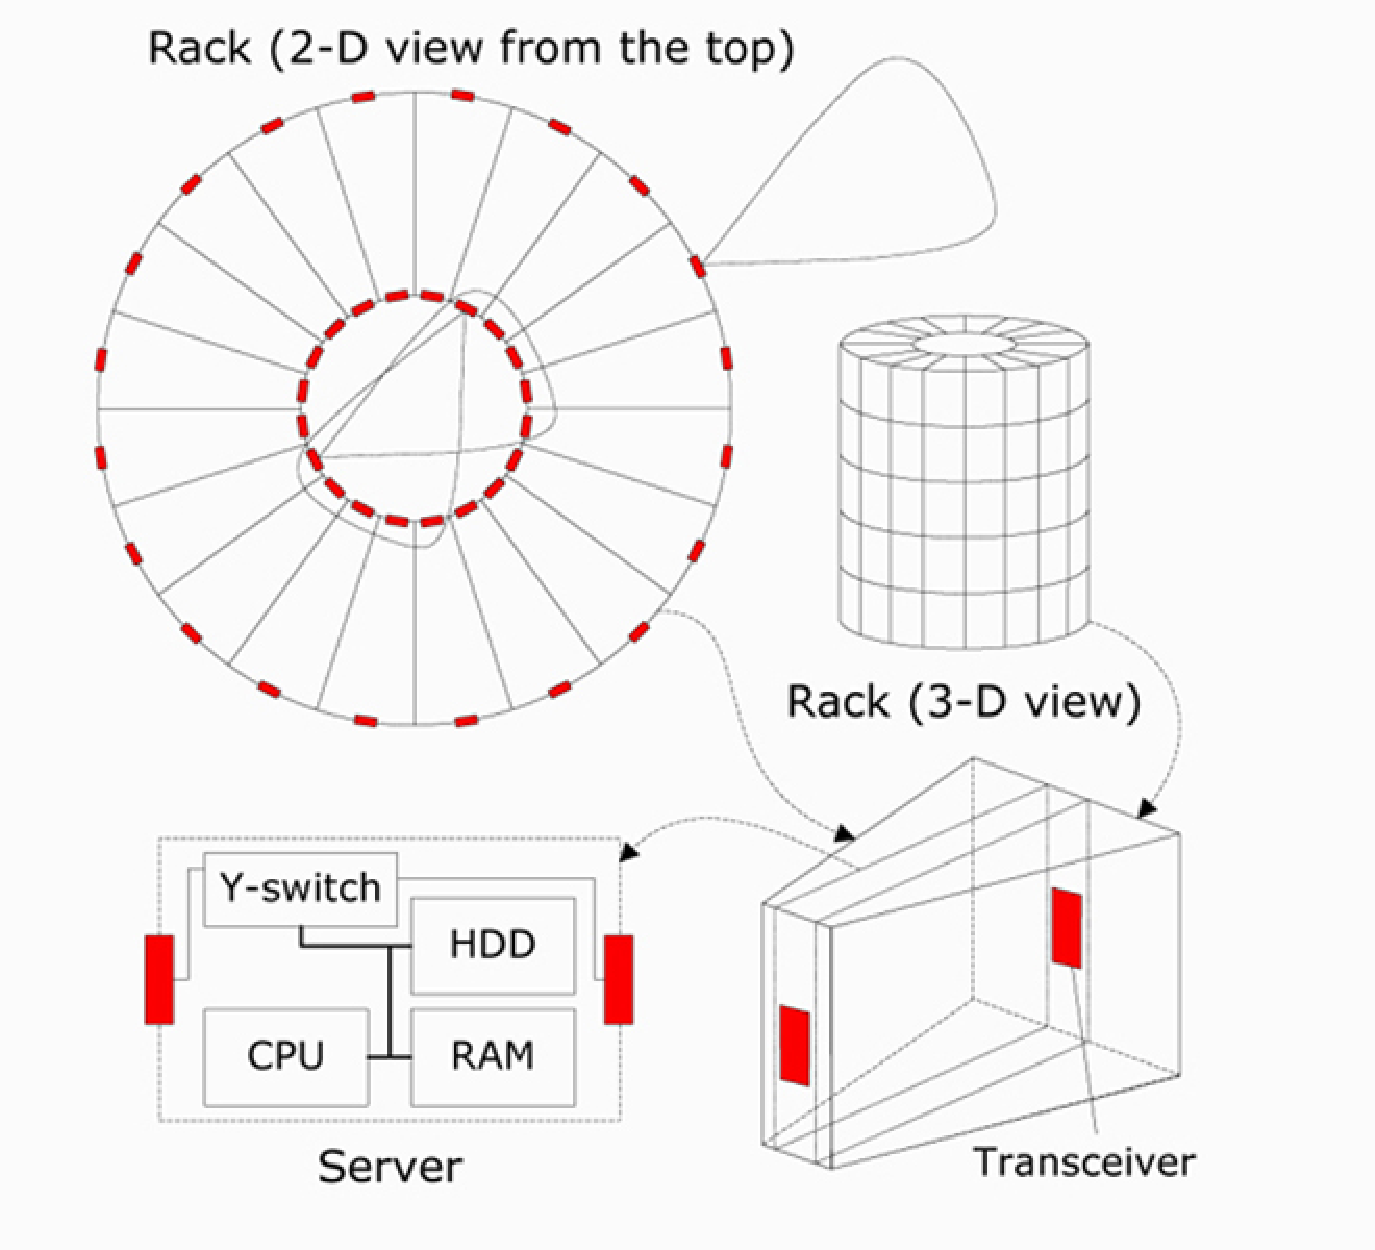
\includegraphics[width=0.4\textwidth]{wirelessdata.pdf}
%\caption{Possible solution: cylindrical racks}
%\label{cylindrical}
%\end{figure}

\begin{enumerate}
  \item electrical
  \item optical
  \item wireless
  \begin{enumerate}
    \item Link Blockage
    \item Radio Interference
  \end{enumerate}
\end{enumerate}

\begin{enumerate}
  \item Apart from the concurrent links, the efficient throughput should be explored. For instance, although the concurrent links are more with larger ceiling height $h$, it can decrease the throughput according to the curves of RSS (or Data Rate) vs. distance as shown in Figure 5.
  \item
  \item
\end{enumerate}

Max concurrent links: Link conflicts (SINR); Greedy scheduling (graph coloring); Assigning radios.


\textbf{"Augmenting Data Center Networks with Multi-gigabit Wireless Links", SIGCOMM 2011}

"The base wired network is provisioned for the \textbf{average case} and can be oversubscribed. Each ToR switch is equipped withe one or more 60GHz wireless devices." "A central controller monitors DC \textbf{traffic patterns}, and switches the beams of the wireless devices to set up flyways between ToR switches that provide \textbf{added bandwidth} as needed." So it is ideal for \textbf{flexible and energy-efficient} data centers.

Problem:
\begin{itemize}
  \item Conflict graph: for $N$ racks and $K$ antenna orientations, the input table is very \textbf{large} with the size of $(NK)^2$, and the propagation conditions are similar, i.e., the table is \textbf{sparse}.
\end{itemize}

For flexible data centers, 60GHz wireless is an attractive choice for its simplify and inexpensive features. On the other hand, 60GHz wireless is a active research area, such as IEEE 802.11ad, WiGig and WirelessHD standards, that are still under exploring on protocols and technology. For data centers, it should be further explored according to the topology and requirements.

Resource Allocation

\textbf{"FairCloud: Sharing The Network In Cloud Computing", SIGCOMM 2012}

\textbf{"NetPilot: Automating Datacenter Network Failure Mitigation", SIGCOMM 2012}

\textbf{"Towards Predictable Datacenter Networks", SIGCOMM 2011}

\end{document}
